\documentclass{article}
\usepackage{amsmath,amsfonts,amsthm,amssymb}
\usepackage{setspace}
\usepackage{fancyhdr}
\usepackage{lastpage}
\usepackage{extramarks}
\usepackage{chngpage}
\usepackage{soul,color}
\usepackage{graphicx,float,wrapfig}
\usepackage{CJK}
\usepackage{algorithm}
\usepackage{algorithmicx}
\usepackage{algpseudocode}
\usepackage{enumitem}
\usepackage{tikz}
\usepackage{authblk}
\usepackage{listings}
\newcommand{\Class}{Operating Systems and Distributed Systems}
\newcommand{\ClassInstructor}{Wei Xu}

% Homework Specific Information. Change it to your own
\newcommand{\Title}{Project 1 Part 2.2}
\newcommand{\DueDate}{Nov 29, 2023}

% In case you need to adjust margins:
\topmargin=-0.45in      %
\evensidemargin=0in     %
\oddsidemargin=0in      %
\textwidth=6.5in        %
\textheight=9.0in       %
\headsep=0.25in         %

% Setup the header and footer
\pagestyle{fancy}                                                       %
\chead{\Title}  %
\cfoot{}                                                                %
\rfoot{Page\ \thepage\ of\ \protect\pageref{LastPage}}                          %
\renewcommand\headrulewidth{0.4pt}                                      %
\renewcommand\footrulewidth{0.4pt}                                      %

% set up lstlistings
\lstset{
    basicstyle          =   \sffamily,
    keywordstyle        =   \bfseries,
    commentstyle        =   \rmfamily\itshape,
    stringstyle         =   \ttfamily,
    flexiblecolumns,
    numbers             =   left,
    showspaces          =   false,
    numberstyle         =   \ttfamily,
    showstringspaces    =   false,
    captionpos          =   t,
    frame               =   lrtb,
    basicstyle          =   \ttfamily,
    numberstyle         =   \ttfamily,
    keywordstyle        =   \color{blue},
    keywordstyle        =   [2] \color{teal},
    stringstyle         =   \color{magenta},
    commentstyle        =   \color{red}\ttfamily,
    breaklines          =   true,
    columns             =   fixed,
    basewidth           =   0.5em,
}

%%%%%%%%%%%%%%%%%%%%%%%%%%%%%%%%%%%%%%%%%%%%%%%%%%%%%%%%%%%%%
% Make title
\title{\textmd{\bf \Title}\\{\large Instructed by \textit{\ClassInstructor}}\\\normalsize\vspace{0.1in}\small{Due\ on\ \DueDate}}
\date{}
\newcommand*{\affaddr}[1]{#1} % No op here. Customize it for different styles.
\newcommand*{\affmark}[1][*]{\textsuperscript{#1}}
\newcommand*{\email}[1]{\textbf{#1}}

\author{%
Fangyan Shi\affmark[1], Chengda Lu\affmark[2], and Yiying Wang\affmark[3]\\
\affaddr{\affmark[1]2021010892 \affmark[2]2021010899 \affmark[3]2020011604}\\
\email{\{\affmark[1]sfy21,\affmark[2]lucd21,\affmark[3]wangyiyi20\}@mails.tsinghua.edu.cn}\\
}
 
\renewcommand\Authands{ and }
%%%%%%%%%%%%%%%%%%%%%%%%%%%%%%%%%%%%%%%%%%%%%%%%%%%%%%%%%%%%%

\begin{document}


\begin{spacing}{1.1}
\maketitle \thispagestyle{empty}
%\cite{}
%%%%%%%%%%%%%%%%%%%%%%%%%%%%%%%%%%%%%%%%%%%%%%%%%%%%%%%%%%%%%
% Begin edit from here

\newcommand{\FIGDIR}{} % This is to be filled by makefile

\section{Experiment Framework}

In this part, we elaborate how we implemented the client11 and server(which is also used for client22), how we solve all issues we met and how to run the codes. Only highlighting points are mentioned.

\subsection{Shared Memory}

This part requires us to develop a mechanism to coordinate multiple processes' requests for server. Since golang isn't designed for this specified purpose, we develop an initial package in \textbf{go-workspace/part2/shmatomicint}. As the name indicates, we can create a shared memory between multiple processes developed by golang and allow atomic operations at the shared memory space. For simplicity, we only open a small space enough for an atomic integer, which can be used to develop larger atomic operations. 

Developing the go package requires cgo. There are C files in \textbf{go-workspace/part2/shmatomicint}, which implements the fundamental mechanism of shared memory. We write a C test file in \\ \textbf{go-workspace/part2/cmd/testC\_shmatomicint}, and running this code will show the effect of atomic integer in C code.

In \textbf{go-workspace/part2/cmd/client21/main.go}, we use the following section of code
\begin{lstlisting}[language=Go]
task_no := shmatomicint.New(shm_name, 0)
for task := task_no.AtomicFetchAdd(1); task < 2000; task = task_no.AtomicFetchAdd(1) {
    // some operations here
}
\end{lstlisting}
to make all processes request for all images only once. Also, all processes have to write the statistic file, so that we can do performance analysis. To achieve writing to the same file by multiple processes as we want, We also utilize the same field of atomic integer.

\subsection{Performance Indicator}

We mainly measures three performance indicators: throughput(or total running time), latency and ongoing requests in the server(which approximately tells us the queue length and CPU utilization). Except latency, the other two are straightforward. We elaborate how we measure latencies in our experiment.

A picture is worth a thousand words. The following figure shows the life cycle of a request, which shows the life cycle of a request on the right and the times we measure on the right.

\begin{figure}[htbp]
    \centering
    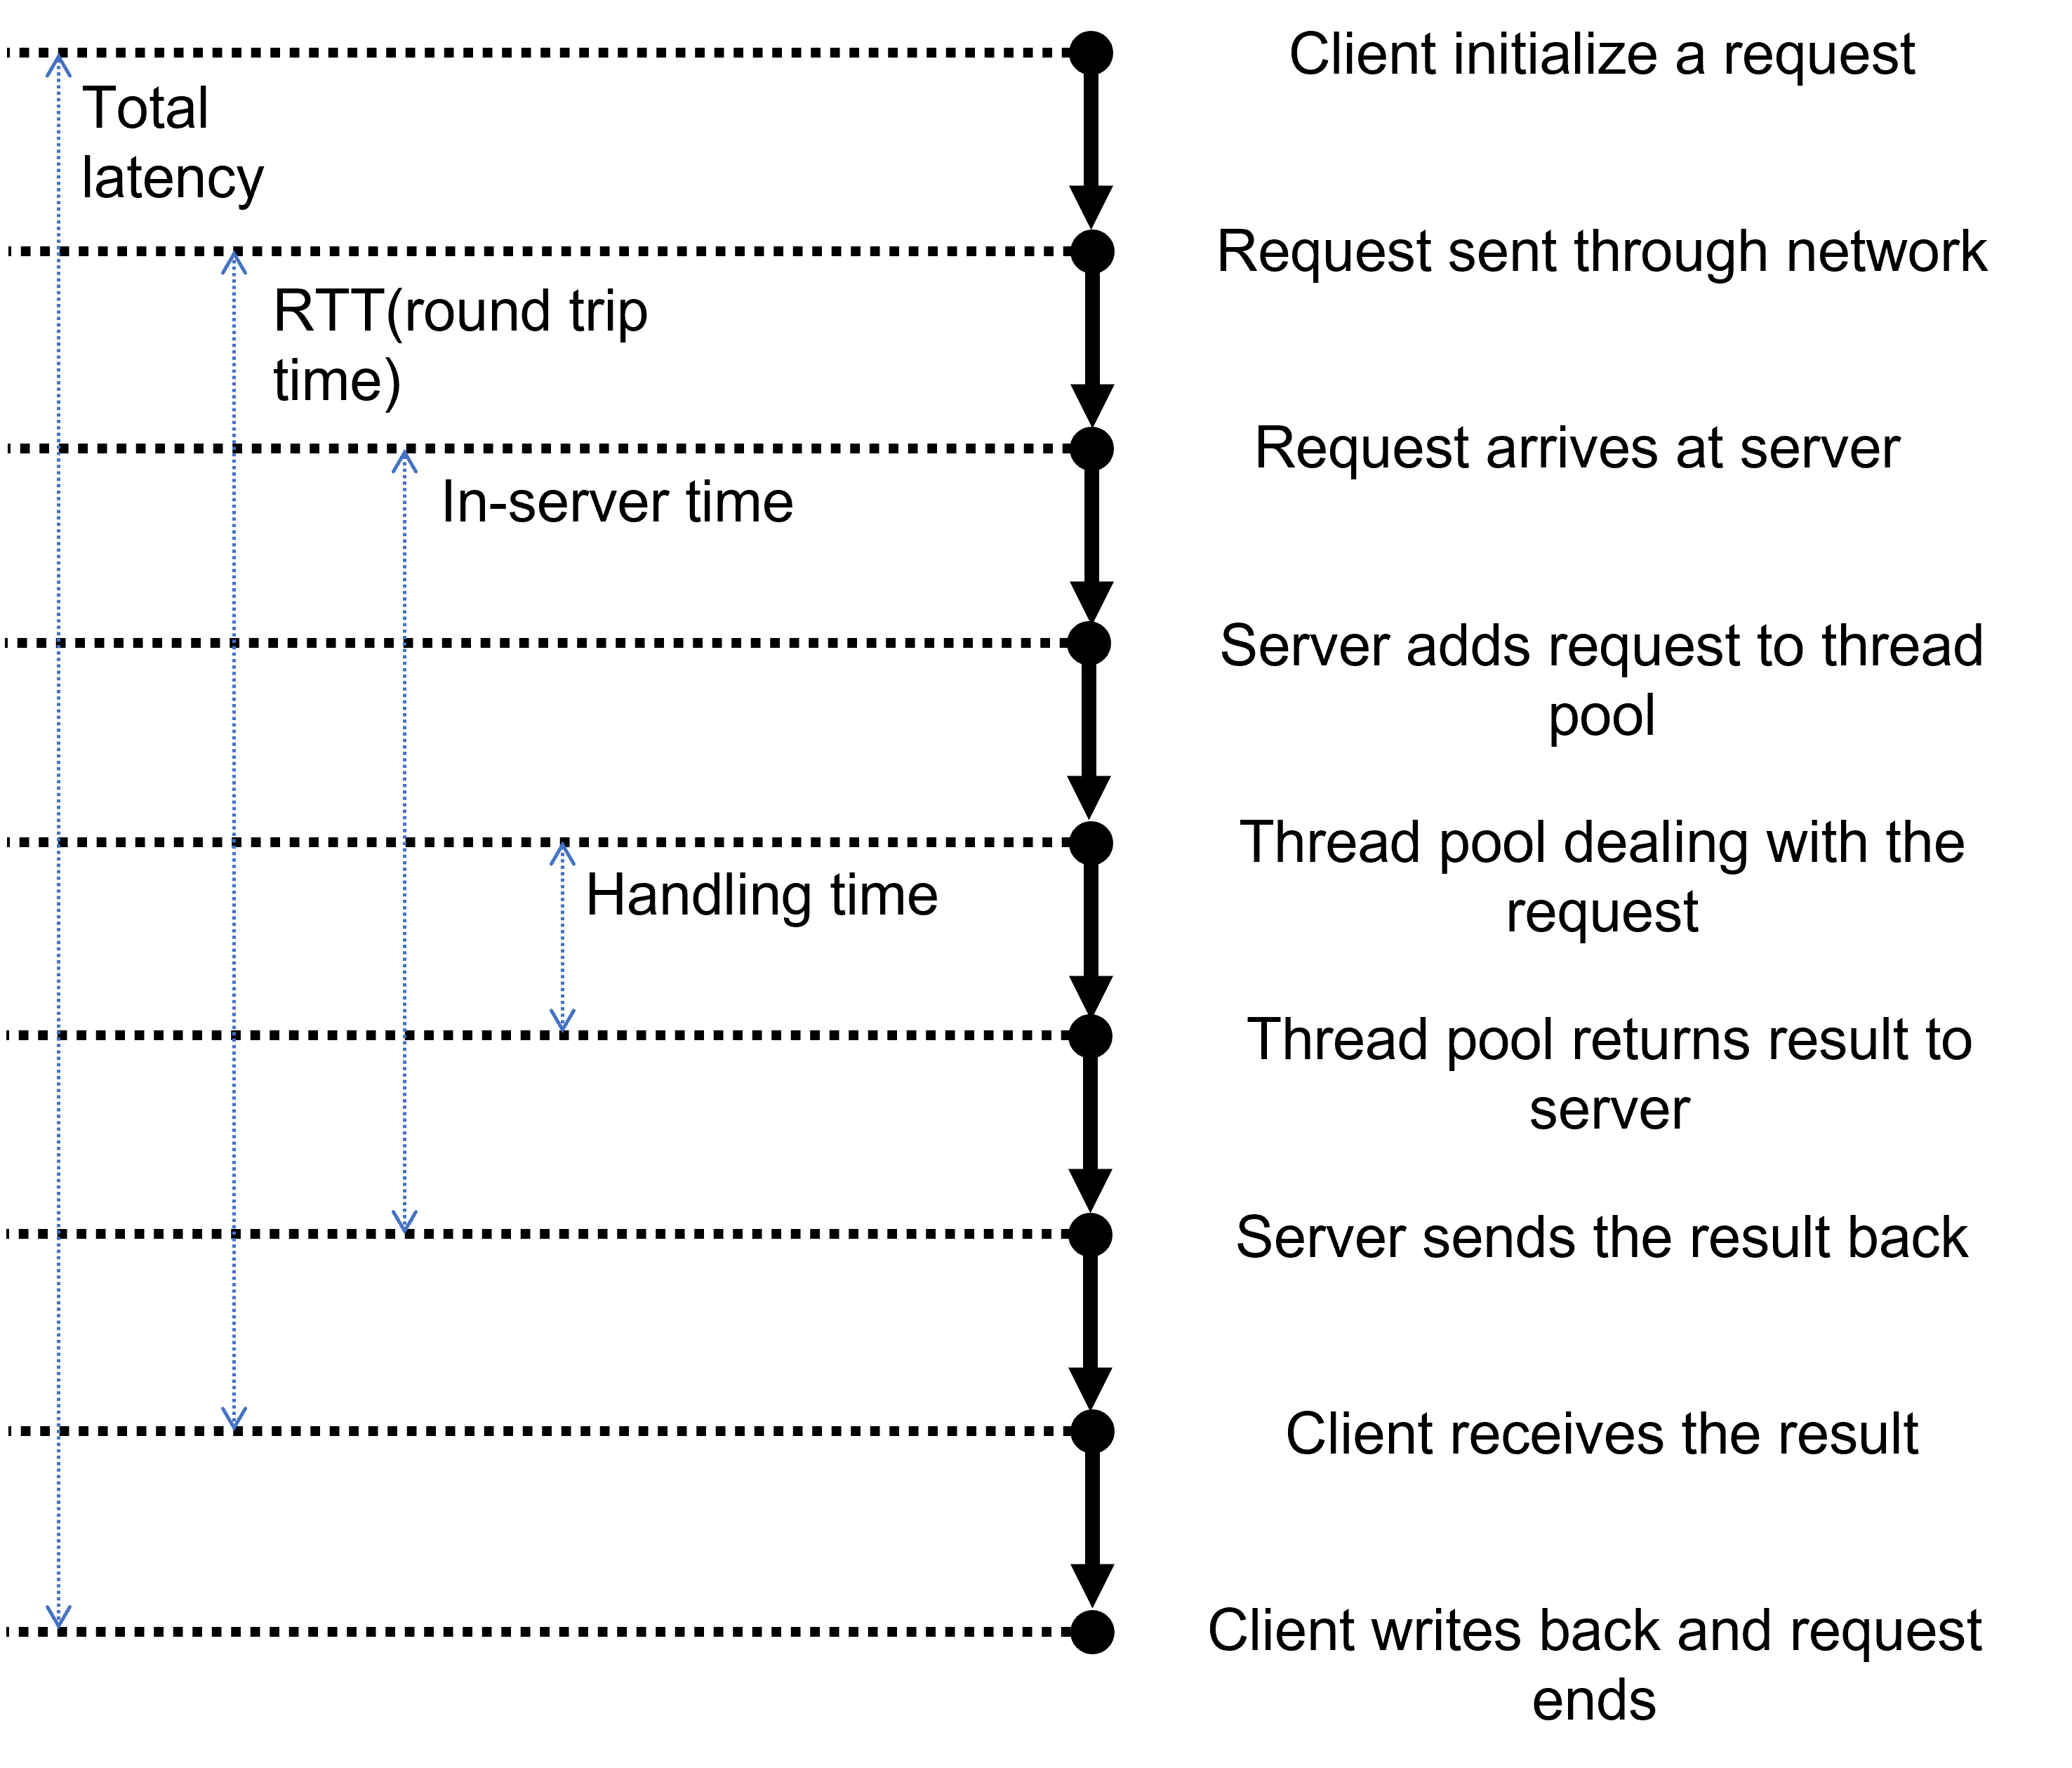
\includegraphics[width=0.5\linewidth]{\FIGDIR/life_cycle.png}
    \label{fig:enter-label}
    \caption{Left: Time Indicators, Right: Life Cycle}
\end{figure}

With the four time indicators, we can further calculate
\begin{itemize}
    \item Network Latency(time spent in the fly) $=$ (RTT) $-$ (In-server Time)
    \item Queuing Time $\approx$ (In-server Time) $-$ (Handling time)
\end{itemize}
These indicators are also important for performance analysis.


\subsection{Let's Run!}

We describe how to use server and client21 commands in this section.

First, build server in directory \textbf{go-workspace/part2/cmd/server} and we will get excutable file \textbf{server}. You need to specify the following parameters to run the server correctly.
\begin{itemize}
    \setlength\itemsep{1pt}
    \item \textbf{-n-t=}: number of working threads in the thread pool.
    \item \textbf{-addr=}: the listening address of the server, e.g., 10.1.0.91:51151.
\end{itemize}

To build client21, run go build for directory \textbf{go-workspace/part2/cmd/client21} and we will get executable file \textbf{client21}. You need to specify the following parameters to run the client correctly.
\begin{itemize}
    \setlength\itemsep{1pt}
    \item \textbf{-n-t=}: number of requesting threads of client.
    \item \textbf{-master}: whether the client is a master process. A master process creates the shared memory integer and used by all clients.
    \item \textbf{-out-dir=}: directory to store the downloaded images.
    \item \textbf{-stats-file=}: file to store the statistics information.
    \item \textbf{-time-file=}: file to store the total running time.
    \item \textbf{-addr=}: Server address to request from.
    \item \textbf{-proc-id=}: The client id for a non-master process. Shall be a integer sequence from 1.
\end{itemize}

\section{Performance Analysis}
We mainly conduct two sets of experiments and we describe them in the following subsections.

\subsection{Experiment set 1}

In this experiment set, we mainly compare the influence of server threads, when number of client threads gives different values. The results are shown by following graphs. We only run single client process and send requests to only one server.

\begin{figure}[htbp]
	\centering
	\begin{minipage}{0.32\linewidth}
		\centering
		\includegraphics[width=0.9\linewidth]{\FIGDIR/part21-throughput.png}
		\label{throuput1}
	\end{minipage}
	%\qquad
	\begin{minipage}{0.32\linewidth}
		\centering
		\includegraphics[width=0.9\linewidth]{\FIGDIR/part21-latency.png}
		\label{latency1}
	\end{minipage}
    \begin{minipage}{0.32\linewidth}
		\centering
		\includegraphics[width=0.9\linewidth]{\FIGDIR/part21-network_latency.png}
		\label{network-latency1}
	\end{minipage} \\
    \begin{minipage}{0.32\linewidth}
		\centering
		\includegraphics[width=0.9\linewidth]{\FIGDIR/part21-speed_up.png}
		\label{speed-up}
	\end{minipage}
    \begin{minipage}{0.32\linewidth}
		\centering
		\includegraphics[width=0.9\linewidth]{\FIGDIR/part21-queue_latency.png}
		\label{queue-latency1}
	\end{minipage}
	%\qquad
	\begin{minipage}{0.32\linewidth}
		\centering
		\includegraphics[width=0.9\linewidth]{\FIGDIR/part21-queue_length.png}
		\label{queue-length1}
	\end{minipage}
    \caption{Experiment set 1 results}
\end{figure}

We can conclude from the figures that
\begin{itemize}
    \item When client threads and server threads increase, the throughput will also increase accordingly. When the number of threads is low, it reaches a good speedup. 
    \item The speedup is generally bounded by $\max\{\text{num\_client\_threads}, \text{num\_server\_threads}\}$, which is to our expectation.
    \item When number of client threads is much greater than that of server threads, we can observer a dramatic increase in latency, and from the figure of queue latency, we know that the queue latency will contribute to most of total latency. However, when we increase the number of server threads, the main part of latency is composed by handling time, which is not shown among the figures above.
    \item Network latency contributes to almost nothing in this task. However, when we flood the server(throughput is high), the network latency will increase in a higher way, compared to the increase of throughput.
\end{itemize}

\subsection{Experiment Set 2}
In this experiment set, we compare the impact of different number of client processes. To make the comparison fair, we fix the number of total working threads, i.e., $\text{num\_client\_threads} \times \text{num\_client\_processes}$ will be a fixed value.

Actually, there isn't much difference when changing the number of client processes. It seems that there will be slightly improvement given more client processes, and we suppose that it might be benefited from the less work on sceduling go routines. However, we discovered that using more client processes will add to a considerable CPU utilization on client machine. Thus, it might not be economic to use more client processes. A lightweight thread will be a better choice.

\begin{figure}[htbp]
    \centering
	\begin{minipage}{0.32\linewidth}
		\centering
		\includegraphics[width=0.9\linewidth]{\FIGDIR/part21-throughput2.png}
		\label{throuput2}
	\end{minipage}
	%\qquad
	\begin{minipage}{0.32\linewidth}
		\centering
		\includegraphics[width=0.9\linewidth]{\FIGDIR/part21-latency2.png}
		\label{latency2}
	\end{minipage}
    \begin{minipage}{0.32\linewidth}
		\centering
		\includegraphics[width=0.9\linewidth]{\FIGDIR/part21-network_latency2.png}
		\label{network-latency2}
	\end{minipage} \\
    \begin{minipage}{0.32\linewidth}
		\centering
		\includegraphics[width=0.9\linewidth]{\FIGDIR/part21-queue_latency2.png}
		\label{queue-latency2}
	\end{minipage}
	%\qquad
	\begin{minipage}{0.32\linewidth}
		\centering
		\includegraphics[width=0.9\linewidth]{\FIGDIR/part21-queue_length2.png}
		\label{queue-length2}
	\end{minipage}
    \caption{Experiment set 2 results}
\end{figure}




% End edit to here
%%%%%%%%%%%%%%%%%%%%%%%%%%%%%%%%%%%%%%%%%%%%%%%%%%%%%%%%%%%%%

\end{spacing}

\end{document}

%%%%%%%%%%%%%%%%%%%%%%%%%%%%%%%%%%%%%%%%%%%%%%%%%%%%%%%%%%%%%